\section{Background and Example}
\label{sec_background}




This section gives a background on how metamodels play a significant role when building software languages and their tooling for a better comprehension of the current work. It then discusses the scenario of co-evolution that arises between metamodels and code, and the need for testing its behavioral correctness. 

\begin{figure*}[tb]
\centering
%\hspace*{-1em}
% \vspace{-5mm}
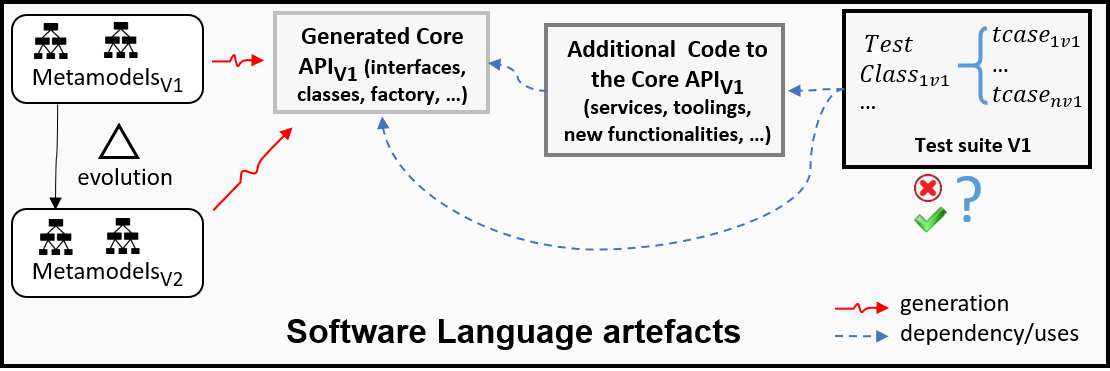
\includegraphics[width=0.9\textwidth]{img/background.png}
%\caption{Artifacts and structure of a software language in the Eclipse platform.}
\caption{Evolution of metamodels and related artifacts of a software language}
\label{fig:SL_useage}
%\vspace{-5mm}
\end{figure*}


\subsection{Key Concepts}

\red{Metamodels are a cornerstone in MDE. It serves to create model instances, constraints, or transformations. 
In our work, we focus on the relation between metamodels and code.
}
Figure \ref{fig:SL_useage} depicts a software language structure and its usage as in practice in the Eclipse platform.  
%
%Metamodels are cornerstones when building a software language and its toolings \cite{van2000domain,gronback2009eclipse}. 
%Metamodels define the aspects of a business domain, i.e. the main concepts, their properties, and relationships between them \cite{cabot2012object}.  
Once the metamodels are carefully defined and validated in a given version. The core API code is generated \cite{steinberg2008emf} consisting of the class implementations of the metamodel classes, a factory and package classes, etc. All this generated code allows parsing the AST of the metamodels' models instances, navigate in it and modify it. 
The generated code is enriched with additional code to offer more advanced functionalities. For instance, methods defined in classes in the metamodel are generated without their bodies, which developers must implement. %This part consists of enriching the generated core API. 
Developers also integrate additional classes to implement advanced functionalities, such as language services like validation and language tooling like an execution engine. %This code is built on top of the generated core API. 
%
Finally, a test suite is added on top of the generated and the additional code to test the implemented functionalities. This can be done manually or with the existing techniques for automated test generation \cite{fraser2011evosuite,mcminn2004search,beyer2022advances}. 

\red{}However, the generated code, additional code and tests hold for a single version of the metamodel. 
\red{With metamodel evolution comes the challenges of co-evolution and its correctness.
For example, when a metamodel evolves, model instances must be co-evolved. One way to check the models' correctness is to rely on the OCL constraints to verify the static semantic of the models \cite{cabot2012object,richters2000validating}. Thus, one can compare the constraints before and after the models' co-evolution.
In our case, when the metamodel evolves}, the API code can be re-generated again. As a consequence, the additional code manually integrated by developers must be co-evolved accordingly as well. 
Unfortunately, there is also no guarantee that the code co-evolution is correct. 
Usually, the test suite is used to identify possible bugs in the new evolved version of the code. In this work, similarly to the practice of regression testing, we leverage the test suites in both the original and evolved versions of the code to check particularly the behavioral correctness of the co-evolution.

\red{Indeed, in regression testing, the goal is to re-run tests after any code changes to ensure that the software still works as intended \cite{leung1989insights,yoo2012regression,wong1997study}. In this paper, we intend to follow a similar methodology by tracing the impacted tests that must be re-run to compare their results before and after code co-evolution.}  
%The next section illustrates these challenges on a real-world use case.  


\red{

\subsection{Motivating Example}
This section introduces a motivating example to illustrate the challenge of metamodel and code co-evolution and testing it. 
% Let us take as an example Ecore project (ref),...
 
 Figure \ref{fig:excerptmodisco} shows an excerpt of the "Modisco Discovery Benchmark" metamodel\footnote{\url{https://git.eclipse.org/r/plugins/gitiles/modisco/org.eclipse.modisco/+/refs/tags/0.12.1/org.eclipse.modisco.infra.discovery.benchmark/model/benchmark.ecore}} consisting of 10 classes in version~0.9.0.
It illustrates some of the domain concepts \texttt{Discovery}, \texttt{Project}, and \texttt{ProjectDiscovery}  used for the discovery and reverse engineering of an existing software system. 
From these metaclasses, a first code API is generated, containing Java interfaces and their implementation classes, a factory, a package, etc. In version 0.11.0, the Modisco  metamodel evolved with several significant changes, among which we find: 1) Renaming the property \emph{totalExecutionTimeInSeconds} to
\emph{discoveryTimeInSeconds} in metaclass \texttt{Discovery}, followed by 2) Moving the property \emph{discoveryTimeInSeconds} (after its renaming) from metaclass \texttt{Discovery} to \texttt{DiscoveryIteration}

%Listing \ref{lis:Modisco_impactedtest_V1} and 
Listing \ref{lis:Modisco_impactedtest_V2} shows a directly impacted test from the class \texttt{DiscoveryImpl\_ESTest} after the evolution of Modisco metamodel. It tests directly the evolved method. 
%
In the class \texttt{DiscoveryIterationImpl\_ESTest} of Modisco 0.11.0, the test shown in Listing \ref{lis:Modisco_indirectimpactedtest_V2} is impacted indirectly by the same change. Indeed, the method \emph{totalExecutionTimeInSeconds} after its rename and move is used in the method \emph{eSet} as shown in Listing \ref{lis:Modisco_eSetmethod_V2}, which is in turn used in the unit test shown in Listing \ref{lis:Modisco_indirectimpactedtest_V2}. It tests indirectly the evolved method. 

The above examples show the direct and indirect impact of the metamodel evolution on the code and on the tests. However, manually tracing the impact of multiple metamodel evolutions at once till the test is tedious, error-prone and time-consuming. In particular, this tracing must be done before and after the metamodel evolution and then to map the traced tests to investigate the code co-evolution correctness. 

The next section presents our contribution for an automated tracing of the tests impacted by the evolution of the metamodel that allows later to check the behavioral correctness of the metamodel and code co-evolution. 

}

%shows a snippet of the generated Java interfaces and classes from the metamodel in Figure \ref{fig:excerptmodisco}. 

\begin{figure*}[tb]
\centering
%\hspace*{-1em}
%\vspace{-5mm}
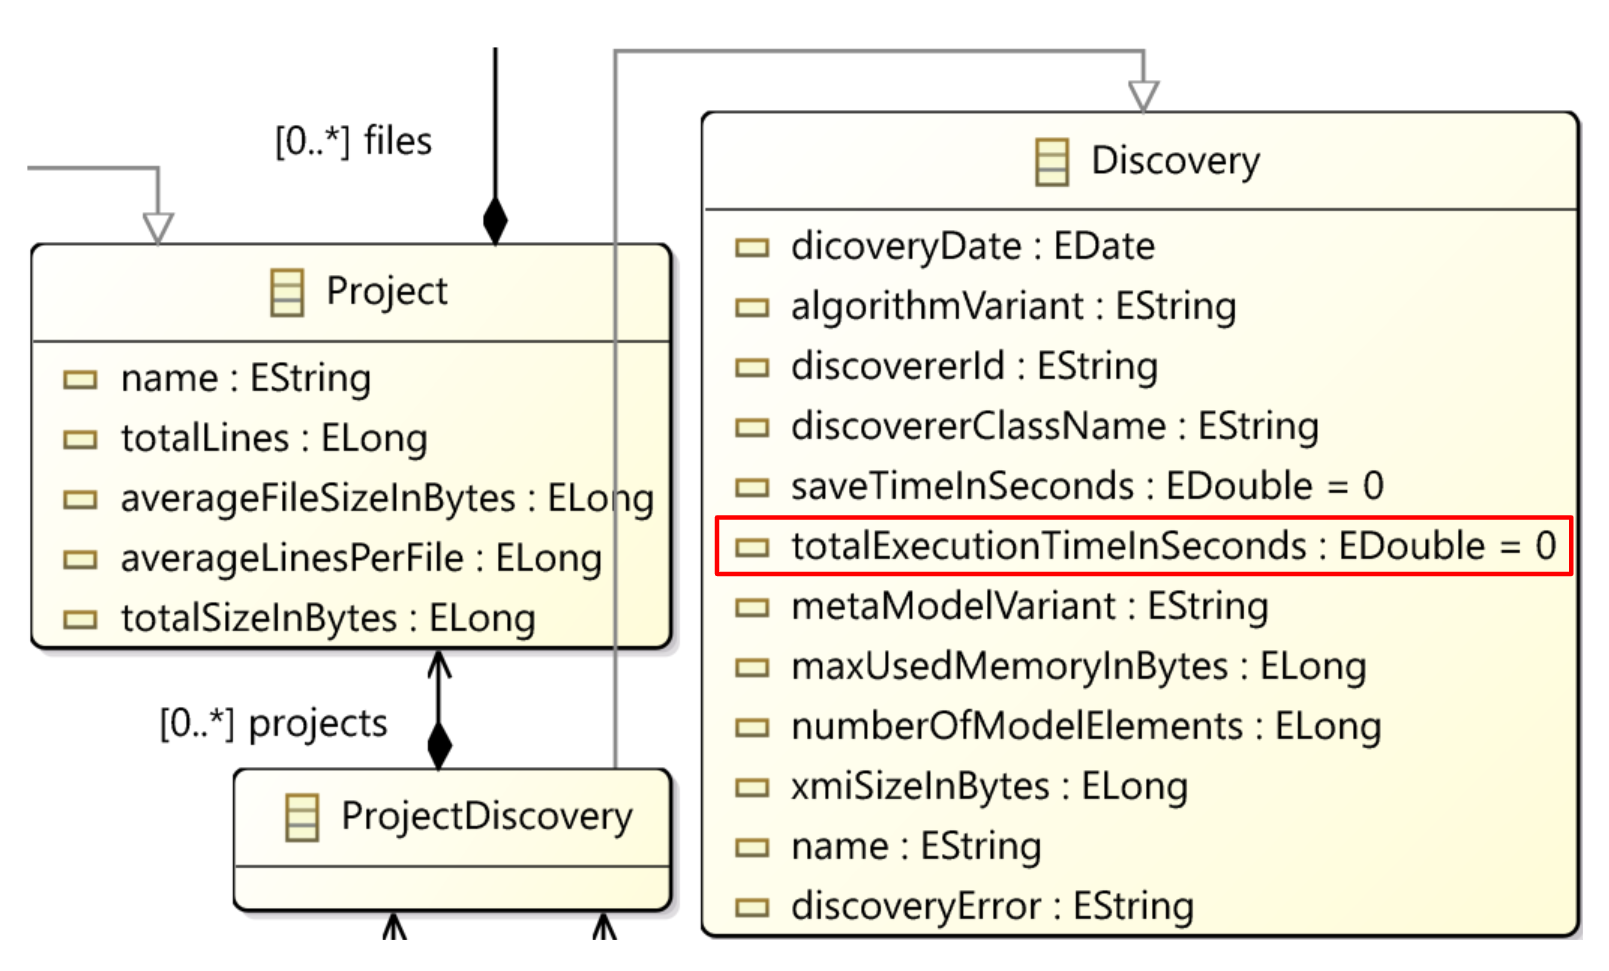
\includegraphics[width=0.7\textwidth]{img/excerptmodisco.png}

\caption{Excerpt of Modisco Benchmark metamodel in version 0.9.0.}
\label{fig:excerptmodisco}
%\vspace{-5mm}
\end{figure*}

\setulcolor{green} 

\begin{comment}

\begin{lstlisting}[language=Java,breaklines=true,mathescape,literate={\-}{}{0\discretionary{-}{}{}},caption=Excerpt of an impacted test in Modisco V1.\label{lis:Modisco_impactedtest_V1}]
   @Test(timeout=4000) public void test000() throws Throwable {
   
      DiscoveryImpl discoveryImpl0=new DiscoveryImpl();
      ...
      assertEquals(0L,discoveryImpl0.getMaxUsedMemoryInBytes());
      assertNull(discoveryImpl0.getAlgorithmVariant()); assertEquals(0.0, (*\ul{discoveryImpl0.getTotalExecutionTimeInSeconds()}*),0.01);
      assertEquals(4,EObjectImpl.ELAST_EOBJECT_FLAG);
      assertTrue(discoveryImpl0.eDeliver());
      assertEquals(0.0, (*\ul{discoveryImpl0.getSaveTimeInSeconds()}*),0.01);
      ...
}
    
    
\end{lstlisting}
\end{comment}


%\setulcolor{green} 

\begin{lstlisting}[language=Java,breaklines=true,mathescape,literate={\-}{}{0\discretionary{-}{}{}},caption=Excerpt of a directly impacted test in Modisco.\label{lis:Modisco_impactedtest_V2}]
   @Test(timeout=4000)
   public void test000() throws Throwable {
    DiscoveryIterationImpl discoveryIterationImpl0 = new DiscoveryIterationImpl();
      ...
      assertFalse(discoveryIterationImpl0.eIsProxy());
      assertEquals(0.0,  (*\ul{discoveryIterationImpl0.getDiscoveryTimeInSeconds()}*), 0.01);
      assertTrue(discoveryIterationImpl0.eDeliver());
      assertEquals(0.0, discoveryIterationImpl0.getSaveTimeInSeconds(), 0.01);
      assertEquals(0L, discoveryIterationImpl0.getMaxUsedMemoryInBytes());
      assertTrue(discoveryIterationImpl0.eDeliver());
      ...
}
    
    
\end{lstlisting}

\begin{lstlisting}[language=Java,breaklines=true,mathescape,literate={\-}{}{0\discretionary{-}{}{}},caption=Excerpt of an indirectly impacted test in Modisco.\label{lis:Modisco_indirectimpactedtest_V2}]
 @Test(timeout = 4000)
  public void test16()  throws Throwable  {
      DiscoveryIterationImpl discoveryIterationImpl0 = new DiscoveryIterationImpl();
      EList<Event> eList0 = discoveryIterationImpl0.getMemoryMeasurements();
      try { 
        discoveryIterationImpl0. (*\ul{eSet(30, (Object) eList0)}*);
        fail("Expecting exception: ClassCastException");
      
      } catch(ClassCastException e) {
        verifyException("org.eclipse.modisco.infra.discovery.benchmark.impl.DiscoveryIterationImpl", e);
      }
      assertEquals(0.0, discoveryIterationImpl0.getSaveTimeInSeconds(), 0.01);
      ...
  }
    
\end{lstlisting}



\begin{lstlisting}[language=Java,breaklines=true,mathescape,literate={\-}{}{0\discretionary{-}{}{}},caption=Excerpt of an impacted method in Modisco.\label{lis:Modisco_eSetmethod_V2}]
@Override
	public void eSet(int featureID, Object newValue) {
		switch (featureID) {
			...
			case BenchmarkPackage.DISCOVERY_ITERATION__DISCOVERY_TIME_IN_SECONDS:
				(*\ul{setDiscoveryTimeInSeconds((Double)newValue)}*);
				return;
			case BenchmarkPackage.DISCOVERY_ITERATION__SAVE_TIME_IN_SECONDS:
				setSaveTimeInSeconds((Double)newValue);
				return;
			case BenchmarkPackage.DISCOVERY_ITERATION__MAX_USED_MEMORY_IN_BYTES:
				setMaxUsedMemoryInBytes((Long)newValue);
				return;
    ...
    }
    
    
\end{lstlisting}

